% !TEX program = xelatex
% 04 스케줄링 최적화 보고서 — SA 기반 자원 제약 정비 스케줄링과 replay 검증
\documentclass[11pt]{article}

\usepackage{kotex}
\usepackage{amsmath}
\usepackage{amssymb}
\usepackage[a4paper,margin=24mm]{geometry}
\usepackage{graphicx}
\usepackage{booktabs}
\usepackage{array}
\usepackage{float}
\usepackage{caption}
\usepackage[table]{xcolor}
\usepackage{enumitem}
\usepackage[colorlinks=true,linkcolor=black,urlcolor=blue,citecolor=black]{hyperref}

\graphicspath{{figures/}{figures/scheduling/}}
\captionsetup{font=small,labelfont=bf}
\setlength{\parskip}{0.4em}
\setlength{\parindent}{0pt}
\renewcommand{\arraystretch}{1.15}
\newcommand{\fig}[3]{\begin{figure}[H]\centering\includegraphics[width=#2\linewidth]{#1}\caption{#3}\end{figure}}

\title{\textbf{정비 스케줄링 최적화 보고서}\\[3pt]
\large — Simulated Annealing 기반 자원 제약 스케줄링과 실제 고장 재현(replay) 검증}
\author{항공엔진 잔여수명(RUL) 예측 기반 정비 스케줄링 최적화 프로젝트}
\date{\today}

\begin{document}
\maketitle

\begin{abstract}
\noindent
본 보고서는 파이프라인의 최종 단계 — 예측 RUL을 정비 마감으로 변환해 \textbf{자원 제약 하에서 스케줄을 최적화}하고,
그 스케줄을 \textbf{실제 고장 시점에 재현(replay)}하여 검증한 결과를 기록한다.
fleet은 통합 test 707엔진(v3 혼합 예측, RMSE 10.90), 계획 지평은 10개 창(창 $=$ 13 cycle), 창당 용량 $K{=}75$(슬랙 1.06)다.

두 개의 핵심 발견이 있다.
\textbf{(1) 목적함수의 사양이 결과를 지배한다}: 예측 낭비를 벌점화한 "효율 목적"의 SA는
좋은 초기해(EDF)를 \emph{능동적으로 파괴}해 고장을 48$\to$100--141로 늘렸고(대리목적 불일치),
조기 배정을 버퍼로 보상한 "강건 목적"의 SA는 마감을 깎지 않은 EDF 해(고장 48)를 그대로 보존했다.
공정 비교 감사(\S4.1) 결과 이 48의 원천은 SA 탐색이 아니라 \textbf{"마진 제거$+$조기 배정"}이며
(같은 마진에서 EDF$=$SA, 배정 변경 0/707) — SA의 기여는 개선이 아니라
\emph{그 해가 강건 목적의 실질 최적임을 대규모 탐색으로 확인}한 것과
\emph{잘못된 목적이 좋은 해를 파괴함을 실증}한 것이다.
\textbf{(2) 예측 품질이 결정 품질로 직결된다}: 같은 강건 SA에서 기본 예측(RMSE 15.0) $\to$ 85대 고장,
v3 예측(10.9) $\to$ \textbf{48대}, Oracle $\to$ 4대 —
EDA 루프의 예측 개선이 \textbf{미정비 고장 37대 감소}라는 물리 지표로 환산되었다.
\textbf{(3) 불확실성 정량화가 휴리스틱 버퍼를 대체한다}: 분위수 회귀(P10)를 마감으로 쓰면
균일 버퍼(강건 SA)의 48대가 \textbf{39대($-19\%$)}로 내려가고, 그 위에 버퍼 보상을 더해도 이득이 없다 —
불확실성이 이미 마감에 흡수된 것이다.
주 지표(고장 수·낭비 수명)는 실제 고장 데이터로 직접 세므로 비용 가정에 의존하지 않는다.
\end{abstract}
\vspace{0.5em}
\begin{center}\fbox{\parbox{0.93\linewidth}{\small
\textbf{대응 노트북:} \texttt{notebooks/04\_optimization.ipynb} (27셀) —
정식화 $\to$ 전략 비교 $\to$ 목적함수 $\to$ \emph{공정 비교 감사} $\to$ P10 $\to$ 예측$\to$결정 사슬 $\to$ 롤링.
감사(SA가 바꾼 배정 0/707대)가 노트북에서 직접 재계산된다.\\
\textbf{파이프라인 위치:} 01 EDA $\to$ 02 전처리 $\to$ 03 예측 $\to$ \textbf{04 스케줄링} $\to$ 05 평가\\
\textbf{선행 문서:} \texttt{rul\_model\_report.pdf} (입력 예측, RMSE 10.90) \quad
\textbf{다음 문서:} \texttt{final\_report.pdf} (전체 종합)
}}\end{center}
\vspace{0.5em}


\tableofcontents
\newpage

% =====================================================================
\section{설정 — 정식화와 평가 규약}
% =====================================================================

\subsection{정식화 (README \S문제 정의 그대로)}

계획 지평을 $T{=}10$개 창(창 $=$ 13 cycle)으로 나누고, 창당 정비팀 용량 $K$를 둔다.
\[
d_i = \left\lceil \widehat{\mathrm{RUL}}_i / 13 \right\rceil - s
\quad(\text{예측 마감, } s{=}\text{안전마진}),\qquad
x_{it}\in\{0,1\},\ \textstyle\sum_t x_{it}\le 1,\ \sum_i x_{it}\le K.
\]
part 4종의 setup 배칭(같은 창에 같은 part를 모으면 setup 절감)이 목적함수를 비분리로 만들어
정확법이 어려워지는 지점이 SA의 담당 영역이다(\texttt{src/pipeline.py}의 다중시작 SA).

\subsection{평가 규약 — replay}

\textbf{계획은 예측으로, 평가는 실제로.}
스케줄 $m_i$를 실제 고장 창 $d^{\text{true}}_i = \lceil \mathrm{RUL}^{\text{true}}_i/13 \rceil$에 재현하여
\begin{itemize}[nosep]
  \item \textbf{미정비 고장 수} (주 지표): $m_i{=}0$ 이거나 $m_i > d^{\text{true}}_i$인 엔진 수
  \item \textbf{낭비 수명}: 제때 정비된 엔진의 $d^{\text{true}}_i - m_i$ 합 (조기 정비가 버린 잔여수명)
  \item 총비용: $C_{pm}{\cdot}$정비 $+ C_{fail}{\cdot}$고장 $+ w{\cdot}$낭비 $+$ setup (참고 지표, $C_{fail}{:}C_{pm}=5{:}1$ 기본)
\end{itemize}
주 지표 둘은 실측 고장 데이터로 직접 세므로 \textbf{비용 가정과 무관}하다.

\subsection{fleet과 규모}

통합 test 707엔진, 예측 $=$ v3 혼합(RMSE 10.90).
예측 마감 분포(마진 0): 창1부터 $[77, 68, 47, 44, 42, 35, 57, 75, 98, 164]$ —
수요가 양끝에 몰려 있고 총 707 vs 슬롯 750(슬랙 1.06)이라 \textbf{용량이 실제로 묶인다}(스케줄링이 자명하지 않은 이유).

% =====================================================================
\section{Simulated Annealing — 개념적 기초}
% =====================================================================

본 절은 SA를 처음 접하는 독자를 위해, 알고리즘의 유래와 각 구성요소가 \emph{왜} 존재하는지를
우리 스케줄링 문제에 직접 대응시키며 설명한다.

\subsection{왜 탐욕적 방법으로는 부족한가 — 국소 최적의 함정}

우리 문제의 해는 "엔진 707대 각각을 어느 창(1--10)에 배정하는가"라는 벡터 하나다.
가능한 배정은 $10^{707}$가지 수준이라 전수 탐색은 불가능하고,
setup 배칭(같은 창에 같은 부품을 모으면 절감) 때문에 한 엔진의 최적 창이 \emph{다른 엔진들의 배정에 의존}한다 —
목적함수가 엔진별로 분리되지 않아 정확법(정수계획)도 무겁다.

가장 단순한 대안은 탐욕적 개선(hill-climbing)이다: 현재 해에서 조금 바꿔 보고, 좋아질 때만 이동한다.
문제는 \textbf{국소 최적(local optimum)}이다 —
"어느 한 엔진을 옮겨도 당장은 나빠지지만, 두세 대를 \emph{함께} 옮기면 크게 좋아지는" 지형에서
탐욕법은 첫 번째 골짜기에 갇혀 멈춘다.
예컨대 배칭 이득을 잡으려면 일시적으로 비용이 오르는 중간 상태를 통과해야 하는데, 탐욕법은 그 언덕을 넘지 못한다.

\subsection{야금학에서 온 아이디어 — 담금질(annealing)}

SA(Kirkpatrick et al., 1983)는 금속 열처리의 \textbf{담금질}을 모사한다.
금속을 고온으로 가열하면 원자들이 활발히 움직이며 나쁜 배열도 자유롭게 오가고,
\emph{천천히} 식히면 원자들이 정렬할 시간을 얻어 낮은 에너지의 균일한 결정 구조에 도달한다.
반대로 급랭(quenching)하면 원자들이 제자리에서 얼어붙어 높은 에너지의 결함 많은 구조가 남는다.

\begin{table}[H]
\centering
\caption{담금질 은유의 3단 대응 — 야금학 $\to$ 최적화 일반 $\to$ 우리 문제}
\label{tab:analogy}
\begin{tabular}{lll}
\toprule
야금학 & 최적화 일반 & 본 스케줄링 문제 \\
\midrule
원자 배열 & 해(solution) & 707차원 배정 벡터 $m$ \\
에너지 $E$ & 목적함수 값 & 스케줄 비용(고장$+$낭비$+$setup) \\
온도 $T$ & 나쁜 해의 수용 관용도 & (동일 — 탐색 제어 변수) \\
가열 후 서냉 & 탐험$\to$수렴 (diversification$\to$intensification) & 초기 큰 이동 허용 $\to$ 후기 미세 조정 \\
급랭(quenching) & 탐욕적 hill-climbing & EDF류 일회성 규칙 \\
결함 있는 급랭 구조 & 국소 최적에 갇힌 해 & 배칭 이득을 못 잡은 스케줄 \\
\bottomrule
\end{tabular}
\end{table}

핵심 통찰: \textbf{좋은 최종 구조를 원하면, 초기에 일부러 나쁜 상태를 허용해야 한다.}
탐욕법이 급랭이라면, SA는 서냉이다.

\subsection{알고리즘 순환과 수용 확률}

SA는 다음 순환을 반복한다 (Modify \& Check for Acceptance):

\begin{enumerate}[nosep]
  \item 현재 해 $m$에서 \textbf{이웃(neighbor)} $m'$을 하나 만든다.
        우리 문제의 이웃 $=$ "엔진 한 대를 다른 창으로 이동" 또는 "두 엔진의 창을 교환"(35\%).
  \item 에너지 변화 $\Delta E = C(m') - C(m)$을 계산한다.
  \item $\Delta E \le 0$(개선)이면 무조건 수용. $\Delta E > 0$(악화)이면 \textbf{확률}
        $P = \exp(-\Delta E / T)$로 수용한다 (Boltzmann 분포에서 유래).
  \item 온도를 낮추고($T \leftarrow \alpha T$) 반복한다.
\end{enumerate}

수용 확률의 직관 — 같은 악화폭 $\Delta E{=}10$이라도 온도에 따라 운명이 다르다:

\begin{center}
\begin{tabular}{rrl}
\toprule
온도 $T$ & $P=\exp(-10/T)$ & 의미 \\
\midrule
100 & $\approx 0.90$ & 거의 수용 — 자유로운 \textbf{탐험} (초기) \\
10 & $\approx 0.37$ & 절반 못 미치게 수용 — 탐험과 수렴의 전환기 \\
1 & $\approx 0.00005$ & 사실상 거부 — 순수 \textbf{내리막 수렴} (말기) \\
\bottomrule
\end{tabular}
\end{center}

즉 온도는 "나쁜 이동을 얼마나 관용할 것인가"의 다이얼이고,
냉각 스케줄은 그 다이얼을 시간에 따라 돌리는 계획이다.
악화폭에도 반응한다: 같은 온도에서 조금 나쁜 이동은 잘 수용되고 크게 나쁜 이동은 드물게 수용된다 —
무작위 재시작과 달리 \emph{지형을 존중하는} 탈출이다.

\subsection{설계 결정 네 가지 — 무엇을 정해야 하고 왜 중요한가}

\begin{itemize}[nosep]
  \item \textbf{초기 온도 $T_0$}: 너무 낮으면 시작부터 탐욕법이 되고(급랭), 너무 높으면 예산을 무작위 방황에 낭비한다.
        원칙적 방법: 무작위 해 표본의 목적값 표준편차 $\sigma(C)$로부터
        $T_0=-\sigma/\ln p$ — "초기에 전형적 악화를 확률 $p$로 수용"하도록 역산 (\S8에서 실제 적용).
  \item \textbf{냉각 스케줄}: 지수형 $T_{k+1}=\alpha T_k$가 표준. $\alpha$가 1에 가까울수록 서냉(탐험 길게),
        작을수록 급랭(빠른 수렴, 국소최적 위험).
  \item \textbf{level length $L$}: 한 온도에서 머무는 반복 수. 온도마다 "그 관용도에서의 평형"에
        가까워질 시간을 주는 것 — 이웃공간 크기에 비례시키는 것이 지침이며,
        \S8에서 $L$이 부족하면 튜닝 결론 자체가 왜곡됨을 실측으로 보인다.
  \item \textbf{종료 기준}: 고정 반복수보다 자연 종료($T$가 수용 불가 수준까지 냉각, 또는 무개선 지속)가 원칙적이다.
\end{itemize}

\subsection{우리 문제에서의 추가 요소}

\textbf{제약 처리}: 이웃 이동이 창 용량($K{=}75$)을 깨뜨릴 수 있다.
처리 전략 3분류(Avoid/Penalize/Repair) 중 우리는 \textbf{Repair} —
초과 배정을 감지해 되돌리므로 평가되는 모든 해가 항상 가용하다.
\textbf{다중시작(multistart)}: SA는 확률적이므로 서로 다른 시작에서 여러 번 실행해 최선을 취한다(강의 Lever 2).
\textbf{휴리스틱 초기화}: 무작위 해 대신 EDF/Latest/grouped 중 최선에서 출발하면
수렴이 빠르고 최종 품질도 좋다(Lever 1) — \S8에서 이 선택이 결과 재현성(분산 0)까지 만드는 것을 본다.

이후 절의 실험은 전부 이 어휘 위에 서 있다:
\S3--\S4는 \emph{목적함수(에너지의 정의)}가 결과를 지배함을 보이고,
\S8은 $T_0\cdot\alpha\cdot L$ 튜닝과 확률적 알고리즘의 통계적 검증을 다룬다.

% =====================================================================
\section{1차 결과 — 효율 SA의 패배라는 발견}
% =====================================================================

먼저 통상적 정식화 — 예측 마감 기준 비용(정비$+$고장$+$\emph{낭비 벌점}$+$setup)을 SA로 최소화 — 를 실행했다(표~\ref{tab:naive}).

\begin{table}[H]
\centering
\caption{전략 비교 (예측 마감: v3, 마진 1창, $K{=}75$) — replay 지표}
\label{tab:naive}
\begin{tabular}{lrrrrr}
\toprule
전략 & 미정비 고장 & 낭비 수명 & setup & 총비용 & 시간 \\
\midrule
Random (5시드 평균) & 279.4 & 1826 & — & 2207 & — \\
\textbf{EDF (마감 순 조기 배정)} & \textbf{78} & 1628 & 36 & 1362 & $<$0.01s \\
Latest (마감 직전 배정) & 100 & 1393 & 36 & 1426 & $<$0.01s \\
Grouped-greedy (배칭 우선) & 150 & 2073 & \textbf{11} & 1569 & 0.01s \\
SA — 효율 목적 (낭비 벌점) & 100 & 1393 & 36 & 1426 & 13s \\
\bottomrule
\end{tabular}
\end{table}

\textbf{효율 SA는 Latest와 같은 해로 수렴했고 EDF에 진다.}
원인은 대리목적 불일치다: 예측 마감 기준 "낭비"를 아끼려면 늦게 배정하는 게 최적이지만,
예측이 과대추정된 엔진(실제가 예측보다 일찍 고장)은 늦은 배정에서 그대로 놓친다.
EDF의 무지성 조기 배정이 오히려 과대추정에 강건했던 것이다.
\emph{예측을 신뢰한 효율 최적화는 예측 오차 앞에서 취약하다} — 이것이 1차 실험의 발견이다.

\fig{O1_strategy_comparison}{0.98}{1차 비교 — 효율 목적의 SA는 Latest에 수렴하며 EDF에 뒤진다(좌: 미정비 고장, 우: 총비용).}
\fig{O2_sa_convergence}{0.6}{SA 수렴 곡선 (multistart best, 8000 iter). 예측-마감 목적 기준으로는 정상 수렴 — 문제는 수렴이 아니라 목적이었다.}

% =====================================================================
\section{강건 SA — 부호 하나로 EDF를 넘다}
% =====================================================================

진단이 처방을 준다: replay 관점에서 \textbf{조기 배정은 낭비가 아니라 예측 오차에 대한 버퍼}다.
목적함수의 낭비 가중치 $w$의 부호를 뒤집어($+0.4 \to -0.3$) 조기 배정을 \emph{보상}하면,
SA는 "예측 마감 준수 $+$ 용량 배분 $+$ setup 배칭"을 유지한 채 여유 용량을 버퍼 확보에 쓴다.

\begin{table}[H]
\centering
\caption{강건 SA vs 효율 SA vs EDF — replay 지표 ($K{=}75$). 감사(\S4.1)에서 추가된 EDF@마진0 행에 주목.}
\label{tab:robust}
\begin{tabular}{lrrrr}
\toprule
구성 & 미정비 고장 & 낭비 수명 & setup & 총비용 \\
\midrule
EDF (마진 1) & 78 & 1628 & 36 & 1362 \\
\textbf{EDF (마진 0)} & \textbf{48} & \textbf{1133} & 40 & \textbf{1212} \\
SA-효율 ($w{=}{+}0.4$, 마진 0) & 141 & 935 & 40 & 1565 \\
SA-효율 ($w{=}{+}0.4$, 마진 1) & 100 & 1393 & 36 & 1426 \\
SA-강건 ($w{=}{-}0.3$, 마진 1) & 78 & 1628 & 36 & 1362 \\
SA-강건 ($w{=}{-}0.3$, 마진 0) & 48 & 1133 & 40 & 1212 \\
\bottomrule
\end{tabular}
\end{table}

\subsection{공정 비교 감사 — SA의 순수 기여 분리}
\label{sec:audit}

초기 서술은 "강건 SA(마진 0) 48이 EDF(마진 1) 78을 이겼다"였다.
그러나 이는 \textbf{마진이 다른 불공정 비교}다(Lecture 13의 공정 비교 원칙 위반 — 통제변수 불일치).
같은 조건에서 분리 감사한 결과(\texttt{scripts/run\_04e\_audit.py}):

\begin{itemize}[nosep]
  \item \textbf{EDF@마진0 단독 $=$ 고장 48·낭비 1133} — SA-강건과 완전 동일.
  \item 강건 목적의 multistart SA는 EDF@마진0을 초기해로 채택한 뒤 $3{\times}8000$회 탐색에서
        \textbf{배정을 단 한 대도 바꾸지 못했다}(0/707, 목적값 702.8 동일).
  \item 즉 \textbf{48의 원천은 SA 탐색이 아니라 "마진 제거 $+$ EDF 조기 배정"}이다.
\end{itemize}

이 감사로 SA의 역할이 정확해진다:
\textbf{(i)~검증자} — EDF@마진0이 강건 목적의 실질 최적임을 24{,}000회 이웃 탐색의 무개선으로 확인
(개선 실패는 여기서 정보다);
\textbf{(ii)~목적 사양의 실증} — 효율 목적($w{>}0$)을 주면 SA가 같은 초기해를 \emph{능동적으로 파괴}해
고장을 48$\to$100--141로 늘린다. 잘 짠 목적은 좋은 해를 보존하고, 잘못 짠 목적은 파괴한다 —
"에너지의 정의가 전부"라는 \S2의 명제가 가장 극적인 형태로 확인된 것이다.

\paragraph{마진의 재해석.}
같은 강건 목적에서 마진 1은 78로 후퇴한다 — 하드 마진은 마감을 깎아 가용 창을 줄이고
(용량 압박 $\to$ 미배정), 마진 0의 EDF는 자연스러운 조기 배정으로 같은 강건성을 공짜로 얻는다.
\emph{이 문제 인스턴스에서는} 강건성이 목적함수 보상조차 필요 없이 "마감을 깎지 말고 일찍 배정하라"로 충분했다.

\fig{O5_robust_frontier}{0.75}{효율--강건 트레이드오프. $w$의 부호가 해의 보존/파괴를 가른다 (좌하단 점 $=$ EDF@마진0 $=$ SA-강건).}

% =====================================================================
\section{예측 품질 $\to$ 결정 품질 — 프로젝트의 완성 사슬}
% =====================================================================

같은 스케줄러(강건 구성 $=$ EDF@마진0 상당, \S\ref{sec:audit})를 고정하고 예측만 바꿔 넣었다(표~\ref{tab:quality}) —
스케줄러가 동일하므로 차이는 전부 예측 품질의 몫이다.

\begin{table}[H]
\centering
\caption{예측 품질 실험 — 강건 SA 고정, 예측만 교체 (replay)}
\label{tab:quality}
\begin{tabular}{lrrr}
\toprule
예측 & test RMSE & 미정비 고장 & 낭비 수명 \\
\midrule
기본 모델 (03, 무튜닝 LGBM) & 15.02 & 85 & 1155 \\
\textbf{v3 혼합 (EDA 루프 최종)} & \textbf{10.90} & \textbf{48} & 1133 \\
Oracle (실제 RUL) & 0 & 4 & 1093 \\
\bottomrule
\end{tabular}
\end{table}

\begin{itemize}[nosep]
  \item \textbf{EDA 루프의 결정 가치}: 예측 RMSE $15.0\to10.9$ 개선이 \textbf{미정비 고장 85$\to$48 ($-44\%$, 엔진 37대)}로 환산된다.
        "왜 예측을 개선했는가"에 대한 스케줄링 언어의 답이다.
  \item \textbf{남은 예측 오차의 비용}: Oracle과의 격차 $48-4=44$대 — 완벽한 예측이면 강건 SA는 사실상 전 fleet을 구한다(4대는 용량·이산화 한계).
  \item 낭비 수명은 세 경우 비슷($\approx$1100--1155) — 개선이 낭비 증가 없이 온 것.
\end{itemize}

\fig{O4_pred_quality_to_decision}{0.62}{예측 품질 $\to$ 미정비 고장 (강건 SA 고정). 기본 85 $\to$ v3 48 $\to$ Oracle 4.}

% =====================================================================
\section{P10 분위수 마감 — 균일 버퍼에서 맞춤 버퍼로}
% =====================================================================

강건 SA의 버퍼 보상($w{<}0$)은 \emph{모든 엔진에 균일}하다. 그러나 예측 오차는 균일하지 않으므로,
오차가 작은 엔진에는 버퍼가 낭비되고 큰 엔진에는 부족할 수 있다.
처방: 같은 v3 특징셋으로 \textbf{분위수 회귀}(LightGBM quantile, $\alpha{=}0.1$)를 학습해
"90\% 확률로 이 시점 전엔 고장 나지 않는다"는 \textbf{엔진별 하한 P10}을 마감으로 쓴다:
$d_i=\lceil \mathrm{P10}_i/13\rceil$ (\texttt{scripts/run\_04d\_quantile.py}).

\paragraph{보정 확인.} test 커버리지 $P(\mathrm{RUL}^{true}\ge \mathrm{P10})=84.2\%$
(명목 90\%보다 다소 낮음 — 절단 시점 상태에 대한 분위수의 알려진 보수성 한계로 정직하게 기록).
엔진별 버퍼(점예측$-$P10)는 평균 8--11 cycle.

\begin{table}[H]
\centering
\caption{P10 마감 replay — 균일 버퍼(점예측$+w{<}0$) vs 맞춤 버퍼(P10)}
\label{tab:p10}
\begin{tabular}{lrrrr}
\toprule
구성 & 미정비 고장 & 낭비 수명 & setup & 총비용 \\
\midrule
점예측 @ 마진0 (기존 최선, EDF$=$SA) & 48 & \textbf{1133} & 40 & 1212 \\
\textbf{P10 마감 (EDF $=$ SA중립 $=$ SA강건, 동일해)} & \textbf{39} & 1264 & 39 & \textbf{1184} \\
SA-효율 @ P10 ($w{=}{+}0.4$) & 64 & 997 & 40 & 1263 \\
Oracle-SA (참조) & 4 & 769 & 40 & 1000 \\
\bottomrule
\end{tabular}
\end{table}

세 가지 판정:
(i)~\textbf{맞춤 버퍼가 균일 버퍼를 이긴다} — 고장 $48\to39$ ($-19\%$), 비용도 $1212\to1184$.
낭비는 $+12\%$(더 이른 정비) — 고장 감소와의 명시적 트레이드오프;
(ii)~\textbf{가설 "P10이 $w{<}0$을 불필요하게 만드는가" $\to$ 예} — P10 위에 버퍼 보상을 더해도 39 그대로.
휴리스틱 버퍼가 원리적 불확실성 정량화로 \emph{대체}되었다;
(iii)~효율 목적은 P10에서도 늦은 배정으로 후퇴(64) — 분위수도 과신하면 안 된다.

감사(\S\ref{sec:audit})와 일관되게, P10 마감에서도 EDF와 SA(중립·강건)는 \textbf{문자 그대로 같은 스케줄}에 도달한다
(배정 차이 0/707) — 마감에 정보가 충분하면 단순 규칙(EDF)으로 충분하고,
SA는 그 해가 개선 불가능함을 확인하는 검증자 역할을 한다.

\paragraph{Oracle 격차의 재분해.}
기존 서술 "격차 44 $=$ 예측 오차의 가격"이 정밀해진다:
\textbf{9대 $=$ 불확실성 정보를 쓰지 않은 가격}(회수됨), \textbf{35대 $=$ 현 예측 모델의 환원 불가능한 가격}.
최종 구성은 \textbf{P10 마감 $+$ 조기 배정(EDF, SA로 최적성 확인)}이다.

% =====================================================================
\section{민감도}
% =====================================================================

\begin{itemize}[nosep]
  \item \textbf{용량 $K$ $\times$ 마진} (효율 목적 기준, 그림~\ref{fig:sens}): 모든 $K$에서 마진 1이 최적(0은 버퍼 부족, 2는 용량 압박) —
        하드 마진의 U자형 한계가 드러난다. 단 이는 \emph{효율 목적} 하의 결과로,
        \S\ref{sec:audit}의 마진0$+$조기배정 구성이 이 딜레마 자체를 우회한다. $K$ 증가는 일관되게 이득(72$\to$90에서 고장 102$\to$88).
  \item \textbf{비용비 $C_{fail}{:}C_{pm}\in\{3,5,10\}$}: 최적 스케줄 불변(고장 100 동일, 비용만 스케일) —
        주 결론이 비용 가정에 의존하지 않음을 확인. 이는 주 지표를 물리량(고장 수)으로 둔 설계의 의도된 결과다.
\end{itemize}

\fig{O3_sensitivity_K_margin}{0.62}{\label{fig:sens}민감도: $K\times$마진 (효율 SA, replay 고장 수).}

% =====================================================================
\section{SA 알고리즘 상세·튜닝·통계 검증 — 강의 방법론 정렬}
% =====================================================================

본 절은 SA의 구성요소 정의, 하이퍼파라미터 튜닝, 결과의 통계적 검증을
강의자료(Day~6 SA, Hyper-Parameter Tuning using SA, Lecture~12 성능평가, Lecture~13 증명과 개선)의 방법론에 맞춰 수행한 기록이다
(\texttt{scripts/run\_04b\_sa\_tuning.py}, \texttt{run\_04c\_stats.py}).

\subsection{개념--적용 대응표: 강의 개념이 실험 어디에 쓰였는가}

강의자료 4종의 개념 각각이 본 실험의 어느 결정·수치로 이어졌는지 추적한다.

\paragraph{Day 6 — Simulated Annealing 원리.}
\begin{table}[H]\centering\small
\begin{tabular}{p{0.28\linewidth}p{0.40\linewidth}p{0.24\linewidth}}
\toprule
강의 개념 & 본 실험 적용 & 결과·위치 \\
\midrule
담금질 vs 급랭 은유 & EDF류 일회성 규칙 $=$ 급랭, SA $=$ 서냉으로 문제 프레이밍 & \S2.2 대응표 \\
Boltzmann 수용 $P{=}e^{-\Delta E/T}$ & 파이프라인·강의식 SA 양쪽의 수용 규칙 & \S2.3 직관표(0.90/0.37/$\approx$0) \\
통계적 $T_0{=}-\sigma(C)/\ln p$ & 무작위 가용해 $R{=}30$ $\to$ $\sigma{=}152.5$ $\to$ $p$별 $T_0{=}299{\sim}1447$ & \S8.2 튜닝의 Factor A \\
지수 스케줄 $T_{k+1}{=}\alpha T_k$ & 튜닝의 Factor B ($\alpha\in\{0.7,0.8,0.9\}$) & 열 추세: 자연종료 하 $\alpha{=}0.7$ 우세 \\
level length $\propto$ 이웃공간 & $L{=}700$ ($707{\times}10$의 10\%) & $L{=}150$ 실패 교훈(\S8.2) \\
자연 종료 (무개선/저온) & $T{<}0.05$ 또는 8-level 무개선 & level 수가 $\alpha$의 비용 응답이 됨 \\
JSSP 이웃(교환) & 이웃 $=$ 엔진 창 이동 / 두 엔진 교환(35\%) & \texttt{\_neighbor} \\
\bottomrule
\end{tabular}
\end{table}

\paragraph{Hyper-Parameter Tuning using SA — 실험 설계.}
\begin{table}[H]\centering\small
\begin{tabular}{p{0.28\linewidth}p{0.40\linewidth}p{0.24\linewidth}}
\toprule
강의 개념 & 본 실험 적용 & 결과·위치 \\
\midrule
완전요인 $p\times\alpha$ & 강의 제시 그리드 그대로 $4\times3{=}12$셀 & 그림 O6 \\
반복 $N{=}10{\sim}15$ ("빠진 조각") & 셀당 $N{=}10$ 독립 시드 & 셀이 분포(mean/std/min/max)가 됨 \\
응답변수: 주$+$부 & 주$=$최종 목적값 / 부$=$level 수$\cdot$수용 이동$\cdot$시간 & $\alpha{=}0.9$ 조기종료 진단에 사용 \\
통제변수 명시 & 동일 문제$\cdot$초기해 방식$\cdot$$t_{end}$$\cdot$목적 고정 & \S8.2 서두 \\
mean$+$\textbf{std} 히트맵 쌍 & 신뢰성 히트맵 병기 & 중간 셀 이봉성($\pm$1553) 발견 \\
행/열 추세 판독(최소 셀 집착 금지) & 열($\alpha$)$\cdot$행($p$) 평균으로 결론 & \S8.2 추세 판독 \\
\bottomrule
\end{tabular}
\end{table}

\paragraph{Lecture 12 — 성능 평가.}
\begin{table}[H]\centering\small
\begin{tabular}{p{0.28\linewidth}p{0.40\linewidth}p{0.24\linewidth}}
\toprule
강의 개념 & 본 실험 적용 & 결과·위치 \\
\midrule
단일 실행의 함정 & 핵심 주장을 그룹당 $N{=}10$ 분포로 재검증 & \S8.3, 그림 O8 \\
FEV (SA$=$반복당 1콜) & 예산 회계: 파이프라인 $3{\times}8000$, 튜닝 level${\times}L$ & \S8.1 \\
수렴 곡선 $=$ 진단이지 증명 아님 & O2/O7을 진단용으로 한정, 증명은 분포·검정으로 & \S3, \S8.2 \\
Success Rate (5\% 이내) & 강건 SA 10/10 $=$ 100\% & 표~\ref{tab:stats} \\
Feasible Rate & Repair로 구조적 100\% & \S8.1 \\
Best/Worst ratio & 1.000 ("매 실행 같은 곳 착지") & 표~\ref{tab:stats} \\
상자그림 비교 & O8 (분포$+$개별 점$+$EDF 기준선) & \S8.3 \\
제약 처리 Avoid/Penalize/Repair & \texttt{\_repair} $=$ Repair; 휴리스틱 초기해는 Avoid 성격 & \S8.1 \\
\bottomrule
\end{tabular}
\end{table}

\paragraph{Lecture 13 — 증명과 개선.}
\begin{table}[H]\centering\small
\begin{tabular}{p{0.28\linewidth}p{0.40\linewidth}p{0.24\linewidth}}
\toprule
강의 개념 & 본 실험 적용 & 결과·위치 \\
\midrule
$H_0$/$H_1$ 명시 & $H_0$: "강건$\cdot$효율 목적은 동일 성능" & \S8.3 \\
게이트키퍼 Shapiro-Wilk/Levene & 분산 0 $\to$ 정의 불가 $\to$ 순서도대로 비모수 분기 & \S8.3 \\
2군: t-test vs Mann-Whitney U & MWU(단측) $p{=}8{\times}10^{-6}$, $H_0$ 기각 & \S8.3 \\
결정론 기준 대비 & vs EDF: Wilcoxon signed-rank $p{=}0.001$, 승률 100\% & \S8.3 \\
공정 비교(동일 예산$\cdot$인스턴스) & 모든 SA 변형 동일 FEV$\cdot$동일 fleet$\cdot$동일 replay & 전체 \\
Lever 1 초기화 & 휴리스틱 초기해 $\to$ 분산 0의 원인 & \S8.3 (무작위 초기 std $\pm$1553과 대비) \\
Lever 2 multistart & $n_{starts}{=}3$ & \S4 \\
Lever 4 적응 파라미터 & 냉각 스케줄 자체가 SA의 적응 파라미터 & \S2.4 \\
Lever 5 이웃 설계 & 이동$+$교환 혼합(35\%) & \S8.1 \\
"알고리즘 교체는 마지막 수단" & 알고리즘은 유지, \textbf{목적함수(\S4)$\cdot$초기화$\cdot$마감 정보(P10, \S6)}를 개선 & $100\to48\to39$ 전 과정 \\
\bottomrule
\end{tabular}
\end{table}

\paragraph{적용하지 않은 개념과 이유 (정직한 경계).}
\begin{itemize}[nosep]
  \item \textbf{AFESO$\cdot$FHT$\cdot$T-ratio}: 성공까지의 평균 FEV류 지표는 실행 간 변동을 전제하는데,
        본 배포 구성은 분산 0(전 실행 동일 해)이라 퇴화한다 — 대신 Best/Worst$\cdot$성공률로 갈음.
  \item \textbf{Performance profile (Dolan--Mor\'e)}: 다중 문제 인스턴스 $\times$ 다중 알고리즘 비교용 도구다.
        본 연구는 단일 fleet 인스턴스이므로 해당 없음(K$\times$마진 스윕은 민감도이지 독립 인스턴스가 아님).
  \item \textbf{Lever 3 재시작$\cdot$Lever 6 하이브리드}: 두 독립 구현이 같은 해에 수렴(\S8.2)해
        탐색이 병목이 아님이 확인되어 투입 근거가 없다. Lever 8(다양성)은 개체군 알고리즘 전용.
  \item \textbf{Kruskal-Wallis(3군 이상)}: 주 비교가 2군(강건 vs 효율)이라 MWU로 충분;
        3군 이상 비교가 필요했다면 KW $\to$ Dunn 사후검정 순서였을 것이다.
\end{itemize}

\subsection{구성요소와 제약 처리}

\begin{itemize}[nosep]
  \item \textbf{수용 기준}: $\Delta E \le 0$ 즉시 수용, 아니면 $P=\exp(-\Delta E/T)$ (Boltzmann).
  \item \textbf{초기 온도 $T_0$ — 통계적 결정}: 무작위 가용해 $R{=}30$개의 목적값 표준편차 $\sigma(C){=}152.5$에서
        $T_0=-\sigma/\ln p$ (초기 수용확률 $p$로 매개화; 예: $p{=}0.9 \Rightarrow T_0{=}1447$).
  \item \textbf{스케줄}: 지수 $T_{k+1}=\alpha T_k$, 온도당 level length $L{=}700$회(이웃공간 $707{\times}10$의 $\sim$10\%).
  \item \textbf{자연 종료}: $T<t_{end}{=}0.05$ 또는 8-level 무개선 — 고정 반복수가 아님.
  \item \textbf{제약 처리 $=$ Repair 전략}: 용량 초과 배정을 감지해 되돌리는 \texttt{\_repair}
        (Avoid/Penalize/Repair 3분류 중 Repair) — 평가되는 모든 해가 구조적으로 가용, Feasible Rate 100\%.
  \item \textbf{비용 단위}: SA는 반복당 목적함수 1회 호출(FEV 1) — 예산·비교는 FEV 기준.
\end{itemize}

\subsection{하이퍼파라미터 튜닝 — 완전요인 $+$ 반복}

단일 실행 비교는 "잡음 대 잡음"이므로(단일 실행의 함정), 완전요인 설계로 튜닝했다:
초기 수용확률 $p\in\{0.6,0.7,0.8,0.9\}$ $\times$ 냉각률 $\alpha\in\{0.7,0.8,0.9\}$, \textbf{셀당 $N{=}10$ 독립 시드}.
통제 변수(공정성): 동일 문제(v3 예측 마감, 마진 0), 동일 초기해 방식(무작위 가용해), 동일 $t_{end}$, 동일 강건 목적.
응답 변수: 주 $=$ 최종 목적값 / 부 $=$ level 수($\alpha$의 비용), 수용 이동 수(탐험량), 실행시간.

\paragraph{선행 교훈 — 탐색 예산이 요인 효과를 오염시킨다.}
1차 시도($L{=}150$, 이웃공간의 2\%)에서는 모든 셀이 수렴 전에 자연 종료되어
"빨리 식을수록 유리"라는 \emph{예산 부족의 왜곡된 추세}가 나타났다(승자 평균 3788).
강의 지침대로 $L$을 이웃공간 비례(700)로 올리자 같은 셀이 2077로 내려오며 진짜 표면이 드러났다 —
level length는 $(p,\alpha)$보다 먼저 확보해야 할 통제 변수다.

\begin{figure}[H]\centering
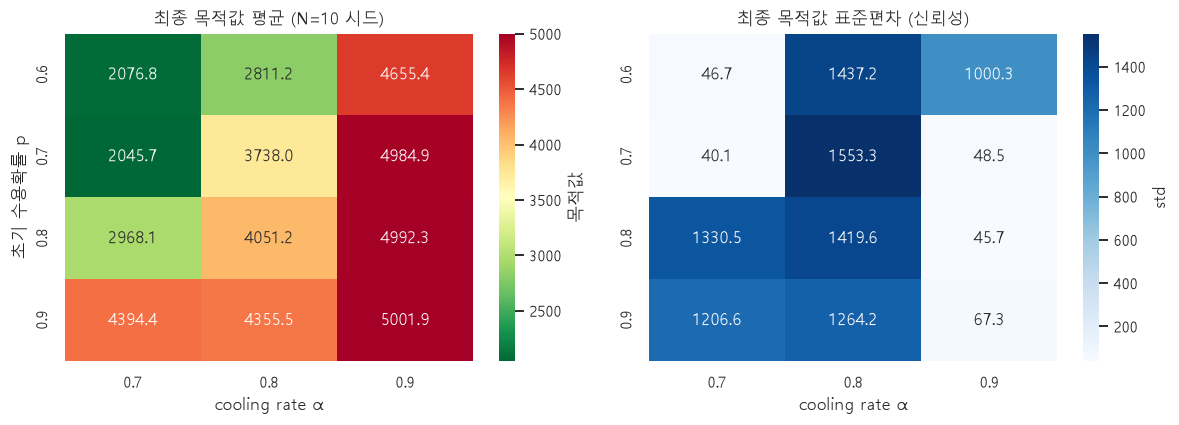
\includegraphics[width=0.95\linewidth]{O6_sa_tuning_heatmaps}
\caption{완전요인 튜닝 — 좌: 최종 목적값 평균($N{=}10$), 우: 표준편차(신뢰성). 최소 셀 하나가 아니라 행·열 추세로 읽는다.}
\end{figure}

\paragraph{추세 판독 (최소 셀 집착 금지).}
열 추세: $\alpha{=}0.7\,(2871) < 0.8\,(3739) < 0.9\,(4909)$ — 자연 종료 하에서 느린 냉각은
고온 방황 중 무개선 정지에 걸려 손해다(level 수 응답이 이를 확인: $\alpha{=}0.9$에서 10--17 level 조기 종료).
행 추세: 낮은 $p$(차가운 시작)가 일관 우세.
std 히트맵은 중간 셀들의 큰 산포($\pm$1200--1550, 이봉성)를 드러낸다 — 평균 히트맵만 보면 놓친다.
승자: $(p{=}0.7,\ \alpha{=}0.7)$, $2045.7\pm40.1$.

\paragraph{배포 실행 — 두 구현의 수렴 일치.}
승자 설정에 휴리스틱 초기화(Lecture 13, Lever 1)를 결합한 배포 실행의 replay는
\textbf{고장 48·낭비 1133·비용 1212} — \S4의 파이프라인 SA-강건(감사 결과 $=$ EDF@마진0)과 \emph{정확히 같은 품질}이다.
서로 다른 두 SA 구현(강의식 level-SA / 파이프라인 SA)이 같은 해 품질에 수렴 —
결론(강건 SA 48)의 구현 독립성이 교차 확인된다.

\begin{figure}[H]\centering
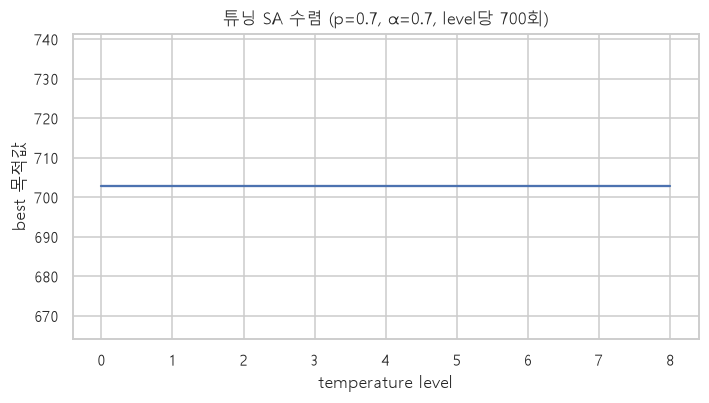
\includegraphics[width=0.6\linewidth]{O7_tuned_sa_convergence}
\caption{튜닝 승자 설정의 수렴 곡선 (level당 700 FEV).}
\end{figure}

\subsection{통계적 검증 — 단일 실행이 아니라 분포로}

핵심 주장(강건 SA $<$ EDF $<$ 효율 SA)을 Lecture 13 워크플로로 검증했다:
그룹별 $N{=}10$ 독립 시드 $\to$ 게이트키퍼 $\to$ 검정.

\begin{table}[H]
\centering
\caption{replay 미정비 고장 수의 분포와 Effectiveness 지표 ($N{=}10$)}
\label{tab:stats}
\begin{tabular}{lrrrrrr}
\toprule
구성 & mean$\pm$std & best & worst & Best/Worst & 성공률(5\%) & Feasible \\
\midrule
SA-강건 ($w{=}{-}0.3$) & $48.0\pm0.0$ & 48 & 48 & \textbf{1.000} & 100\% & 100\% \\
SA-효율 ($w{=}{+}0.4$) & $100.0\pm0.0$ & 100 & 100 & 1.000 & 100\% & 100\% \\
EDF (결정론) & 78 & — & — & — & — & 100\% \\
\bottomrule
\end{tabular}
\end{table}

\begin{itemize}[nosep]
  \item \textbf{게이트키퍼}: 두 분포 모두 분산 0(상수) $\to$ Shapiro-Wilk 정의 불가 $\to$ 강의 순서도대로 \textbf{비모수 분기}.
  \item \textbf{검정}: Mann-Whitney U(단측, 강건$<$효율) $p=8.0\times10^{-6}$ — $H_0$(두 목적함수 동일 성능) 기각.
        vs EDF: 승률 100\%(10/10), Wilcoxon signed-rank $p{=}0.001$.
  \item \textbf{분산 0의 원인}: 결정론적 휴리스틱 초기화(Lever 1)에서 출발한 SA가
        강건 목적에서는 초기해를 전혀 바꾸지 않고(\S\ref{sec:audit}: 0/707), 효율 목적에서는 매 시드
        같은 방향으로 파괴하기 때문 — 무작위 초기화의 튜닝 실행(std 최대 $\pm$1553)과 극명한 대비.
        따라서 이 검정은 실질적으로 \emph{두 목적함수의 비교}이며, 헤드라인 48이 확률적 행운이
        아님(10/10 재현)과 목적 사양의 효과가 실재함을 함께 보인다.
\end{itemize}

\begin{figure}[H]\centering
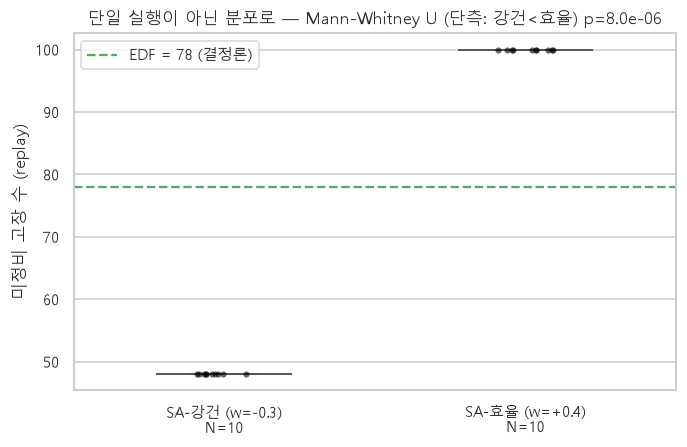
\includegraphics[width=0.6\linewidth]{O8_stat_validation}
\caption{분포 비교 — SA-강건 vs SA-효율 ($N{=}10$, 점$=$개별 실행), 점선$=$EDF@마진1(78).}
\end{figure}

% =====================================================================
\section{확장 실험 — 롤링 재계획(rolling horizon)}
% =====================================================================

지금까지의 설정은 $t{=}0$에 한 번 계획하고 끝나는 \emph{정적} 계획이다.
실제 운영은 매 창마다 새 센서 데이터가 쌓이고, 그때마다 재예측$\cdot$재계획할 수 있다.
이 적응의 가치를 측정했다 (\texttt{scripts/run\_04f\_rolling.py}).

\paragraph{테스트베드 설계.}
test 엔진은 절단 이후 데이터가 없어 재예측 시뮬레이션이 불가능하므로,
\textbf{run-to-failure 전체 궤적을 가진 valid 엔진 178대}(분리-train 미학습)를 쓰고
모델(점예측 v3$\cdot$P10)을 분리-train으로만 재학습했다(누수 차단).
특징이 전부 인과적(past-only; 스파이크 주입 테스트로 검증)이므로
"cycle $t$ 절단 시점의 예측 $=$ 전체 궤적의 $t$행 예측"이 성립해 프리픽스 재계산 없이 시뮬레이션이 가능하다.
초기 나이 $=$ 수명의 $U(0.45,0.90)$(시드 3개), $T{=}10$창, $K{=}19$(슬랙 1.06 동일),
정답 규칙은 본 replay와 동일(죽음 창 $D_i{=}\lceil$잔여$_0/13\rceil$, 정비 창 $\le D_i$면 on-time).
롤링은 매 창 시작 시 생존$\cdot$미정비 엔진을 현재 나이의 특징으로 재예측 $\to$ EDF 재계획 $\to$
이번 창 배정분만 확정 정비한다.

\begin{table}[H]
\centering
\caption{정적 vs 롤링 — 미정비 고장 수 (valid 178대, 시드 42; 괄호는 3시드 mean$\pm$std)}
\label{tab:rolling}
\begin{tabular}{lrrr}
\toprule
 & 점예측 & P10 & Oracle \\
\midrule
정적 (1회 계획) & 22 & 19 \;(24.0$\pm$5.1) & 0 \\
\textbf{롤링 (매 창 재예측$\cdot$재계획)} & \textbf{3} & \textbf{2 \;(1.7$\pm$0.9)} & 0 \\
\bottomrule
\end{tabular}
\end{table}

\begin{figure}[H]\centering
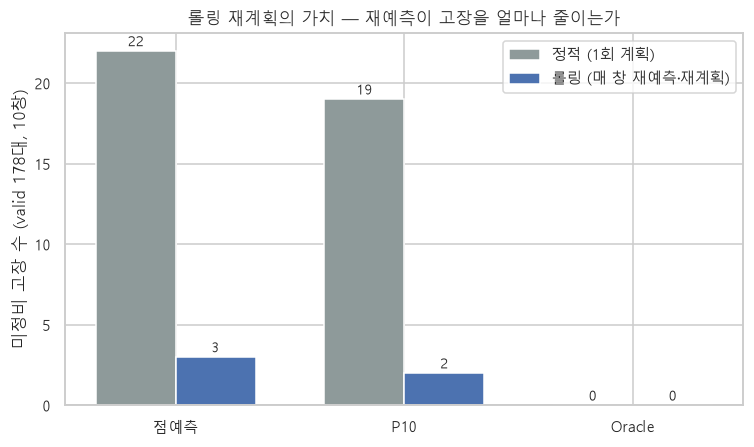
\includegraphics[width=0.62\linewidth]{O9_rolling_vs_static}
\caption{롤링 재계획의 가치 — 재예측이 예측 오차 고장의 $\sim$93\%를 회수한다.}
\end{figure}

네 가지 판정:
\begin{enumerate}[nosep]
  \item \textbf{적응이 예측 오차 비용의 $\sim$93\%를 회수한다}: 정적-P10 $24.0\pm5.1 \to$ 롤링-P10 $1.7\pm0.9$ (3시드).
        낭비도 동반 감소(4128$\to$3935 cyc) — 트레이드오프가 아니라 동시 개선.
  \item \textbf{왜 되는가 — EDA와의 연결}: 열화 말기로 갈수록 신호가 강해진다(onset 이후 오차 급감,
        EDA 보고서 \S핵심 발견). 정적 계획은 신호가 약한 초기 예측의 오차에 \emph{잠기지만},
        롤링은 엔진이 위험해질수록 정확해지는 재예측으로 매 창 수정한다 — 정확도가 필요한 순간과
        정확도가 생기는 순간이 일치한다.
  \item \textbf{동적 설정에서는 재예측이 불확실성 정량화를 대체한다}: 롤링-점예측(3--5) $\approx$ 롤링-P10(1--3).
        \S6의 P10 이득은 \emph{단발 계획} 상황(예: 본 test fleet 설정)에 집중되고,
        재계획이 가능하면 그 역할을 적응이 흡수한다 — \S6 대체 관계의 동적 버전.
  \item \textbf{Oracle은 두 모드 모두 0}: 이 테스트베드의 모든 고장이 예측 오차 기인임을 확인 —
        롤링은 그 비용을 거의 전부 회수한 것이다.
\end{enumerate}

\paragraph{한계.}
valid 테스트베드(178대)는 본 test fleet(707대)과 다르며 초기 나이가 합성 분포다;
창 단위 granularity; 재계획 비용(계획 변경의 운영 마찰) 미반영.
그럼에도 방향은 명확하다: \emph{예측 기반 정비의 실전 가치는 한 번의 좋은 예측보다
"신호가 강해질 때마다 다시 보는" 운영 설계에서 나온다.}

% =====================================================================
\section{결론과 산출물}
% =====================================================================

\paragraph{결론.}
\begin{enumerate}[nosep]
  \item \textbf{목적함수 사양이 전부다}: 효율 목적($w{>}0$)의 SA는 좋은 초기해(EDF)를 능동적으로 파괴해
        고장을 48$\to$100--141로 늘린다 — 예측 오차를 무시한 정식화의 함정.
  \item \textbf{공정 비교 감사로 정정된 사실}(\S\ref{sec:audit}): 고장 48의 원천은 SA 탐색이 아니라
        \textbf{마진 제거 $+$ EDF 조기 배정}이다(EDF@마진0 $=$ SA, 배정 변경 0/707).
        SA의 기여는 이 해가 강건 목적의 실질 최적임을 24{,}000회 탐색으로 \emph{검증}한 것.
  \item \textbf{예측$\to$결정 사슬 정량화}(스케줄러 고정): RMSE 15.0$\to$10.9 $=$ 고장 37대 감소; Oracle 격차 44대.
  \item 주 지표는 비용 가정과 무관(비용비 민감도에서 스케줄 불변).
  \item \textbf{통계적으로 검증됨}: $N{=}10$ 시드 재현 10/10(분산 0), 목적함수 간 Mann-Whitney U $p{=}8{\times}10^{-6}$ —
        완전요인 튜닝($p\times\alpha$, 셀당 10시드)과 별도 구현(강의식 level-SA)의 수렴 일치까지 확인.
  \item \textbf{최종(정적): P10 분위수 마감이 휴리스틱 버퍼를 대체} — 고장 $48\to\mathbf{39}$($-19\%$), 비용 $1212\to1184$;
        P10에서도 EDF$=$SA(동일해). Oracle 격차 분해 완성(9 $=$ 불확실성 미활용, 35 $=$ 예측 오차의 환원 불가능분).
  \item \textbf{확장(동적): 롤링 재계획이 예측 오차 비용의 $\sim$93\%를 회수} — 정적 $24.0\pm5.1 \to$ 롤링 $1.7\pm0.9$
        (valid 테스트베드, 3시드). 재예측 가능 환경에서는 적응이 P10의 역할까지 흡수한다.
\end{enumerate}

\paragraph{산출물.}
\texttt{scripts/run\_04\_scheduling.py}(전략$\cdot$민감도 배터리),
\texttt{run\_04b\_sa\_tuning.py}(완전요인 튜닝), \texttt{run\_04c\_stats.py}(통계 검증),
\texttt{local\_experiments/results/sched\_ckpt/}(스케줄$\cdot$요약 JSON),
그림 O1--O8.
정식화$\cdot$알고리즘은 \texttt{src/pipeline.py} 재사용(EDF/greedy/다중시작 SA/replay).

\paragraph{남은 과제.}
분위수 보정 개선(커버리지 84\%$\to$명목 90\%; conformal 보정 등),
롤링 재계획의 실전화(재계획 비용$\cdot$부분 확정 계획), 부품 재고 제약의 명시적 추가.

\vspace{1em}
\hrule
\vspace{0.6em}
\small
\textbf{근거.} \texttt{rul\_model\_report.tex}(v3 예측, RMSE 10.90), \texttt{README.md}(정식화), \texttt{src/pipeline.py}(알고리즘).
파이프라인 SA 설정: 다중시작 3(Lever 2), 8000 iter, $T_0{=}10$, 냉각 0.997, 이웃 $=$ 창 변경/교환, 초기해 $=$ EDF/Latest/grouped 중 최선(Lever 1).

\textbf{참고문헌.}
강의자료: Introduction to Simulated Annealing (Lecture 6, Summer 2026);
Hyper-Parameter Tuning in Simulated Annealing;
Metaheuristics Performance Assessment (Lecture 12);
Proving and Improving Algorithm Performance (Lecture 13).
문헌: Zapfel, Braune \& B\"ogl (2010) \emph{Metaheuristic Search Concepts};
Halim, Ismail \& Das (2021) Performance assessment of the metaheuristic optimization algorithms, \emph{Artif.\ Intell.\ Rev.};
Dolan \& Mor\'e (2002) Benchmarking optimization software with performance profiles, \emph{Math.\ Program.}

\end{document}
